\section{HexGANFuzzer Framework}
In this section, we describe our methodology and the main aspects of the HexGANFuzzer framework as depicted in Fig. \ref{FigHexGANFuzzer_model}. Firstly, we preprocess message frames captured from the ICS as the training data of the deep adversarial learning model established. Secondly, 
the adversarial network of the HexGANFuzzer framework is composed of 
a generative model and a discriminant model, which generates fake but plausible data via an adversarial learning process for future fuzz testing. %, and a specific model is obtained by training and retraining the model with the acquired data. Finally, a series of performance metrics are put forward to evaluate our model.

 
\begin{figure}[htbp]   %  插入一栏图片
	\centering 
	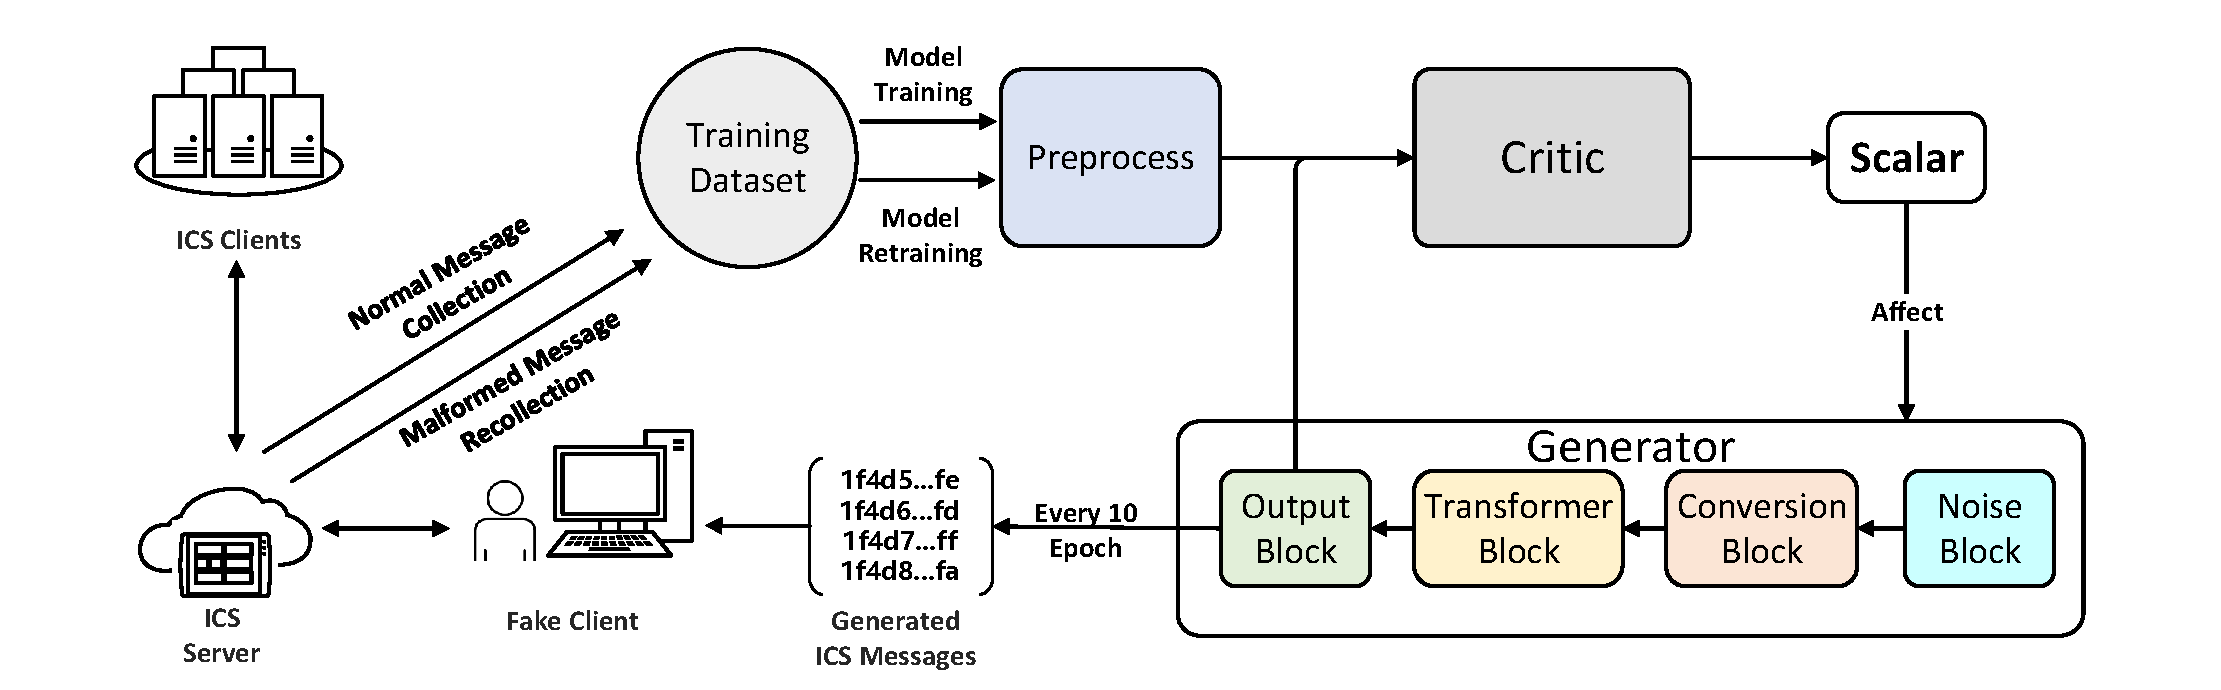
\includegraphics[width=\textwidth]{Figure/FigHexGANFuzzer_model.eps}
	\caption{The framework of HexGANFuzzer}
	\label{FigHexGANFuzzer_model}
\end{figure}

% first acquire a large number of communication data from the ICS to be tested and then
\subsection{Preprocessing of ICP Message Frames}
%diverse test cases, reach high code coverage and
In order to get desirable fuzzing results, data preprocessing is a necessary part. There are two steps in preprocessing: \textbf{Message Frame Clustering} and \textbf{Data Conversion}.

\subsubsection{\textbf{Message Frame Clustering}}
After message frames collection, there are many ICPs' message frames of different lengths. We adopt the Length Clustering method to preprocess the data frames. %It is noted that most message frames with the same length share the same frame type.
First, we gather the data frames which have the same length. %In order not to get too many groups of data frames, 
Groups whose quantity is less than a threshold (e.g. 5000) will be moved to the longer adjacent group, while groups contain more data than the threshold are left unchanged.  %In such a way, there may be message frames with different lengths in one group.
After clustering, the maximum length of message frames of every group will be the standard length and message frames whose length is less than the maximum length will be added special token `u' at the end of them.

\subsubsection{\textbf{Data Conversion}}
The raw data frame of most protocols is hexadecimal, which can not be fed into the model directly. So after clustering, the hexadecimal data frames will be mapped into the digital vectors. The vocabulary we use is as followed:
\begin{equation}
\textit{\textbf{0 1 2 3 4 5 6 7 8 9 a b c d e f u}}
\end{equation}
%The size of the vocabulary is 17, there are ten digits and seven hexadecimal characters according to the hexadecimal message frames and the supplement token `u'.
Based on the vocabulary, message frames $x \in R^{seq\_size \times 1}$ were converted into one hot vector $X \in R^{seq\_size \times 17}$(seq\_size is the maximum length of the current group), and one-hot vectors of real message frame will be the input of the critic.



\subsection{Model Architecture}
\label{sec:model_design} 
As Fig. \ref{FigHexGANFuzzer_model} shows, our model consists of a generator and a critic. 
%, which is the same as a WGAN model
The generator is born to generate the fake message frames and the critic will evaluate the Wasserstein distance. The Wasserstein distance is the minimum cost of transporting mass in converting the data distribution $q$ to the data distribution $p$. During the training, the Wasserstein distance between real message frame distribution and fake message frame distribution will be shortened so that our model grasps specifications of ICPs' grammar.

\subsubsection{\textbf{Generator}}
\begin{figure}[t]   %  插入一栏图片
	\centering 
	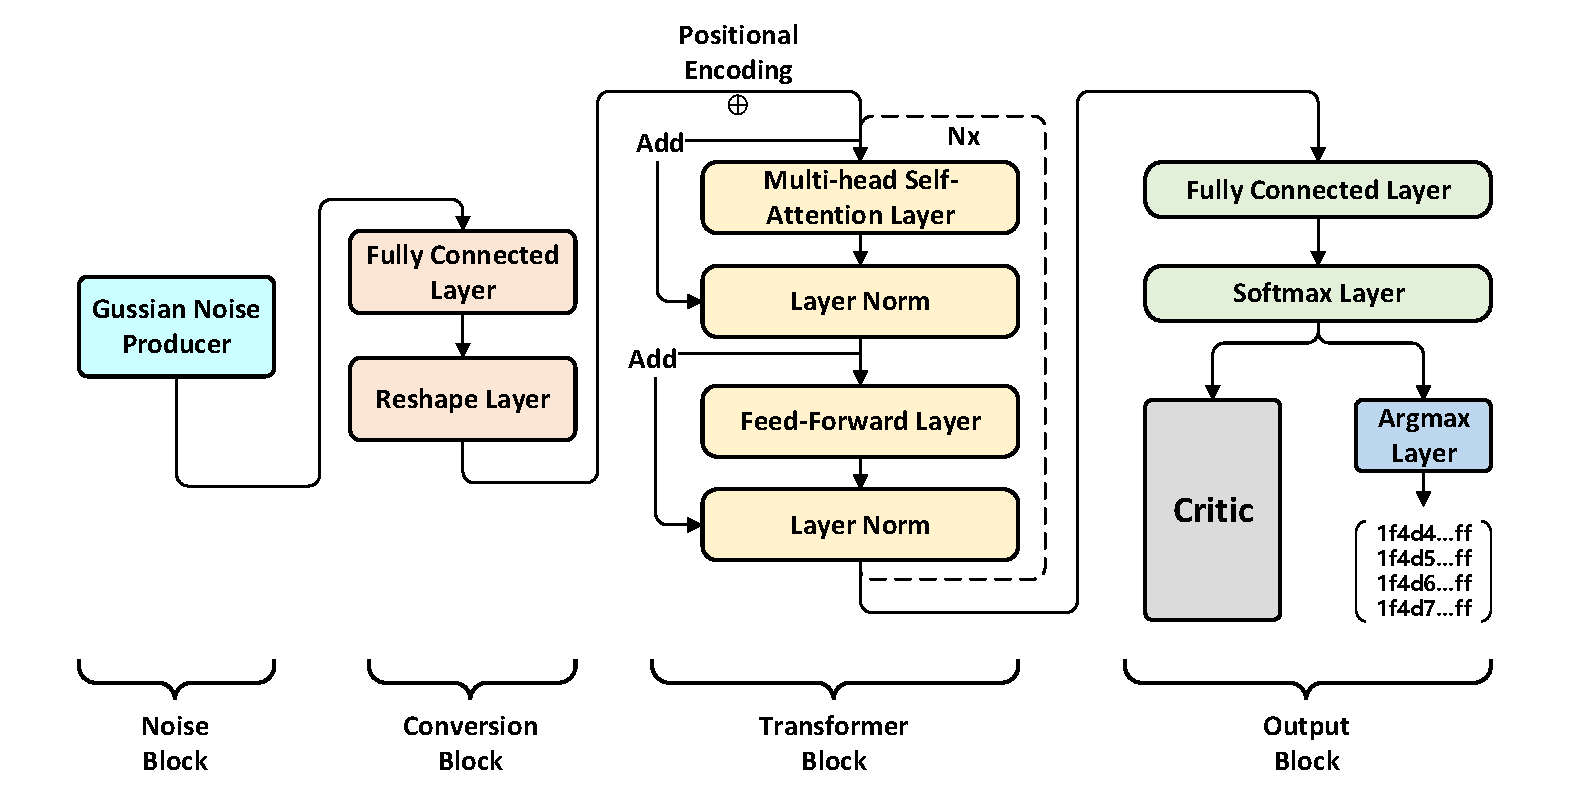
\includegraphics[width=\textwidth]{Figure/FigHexGANFuzzer_Generator.eps}
	\caption{Generator Network}
	\label{FigHexGANFuzzer_Generator}
\end{figure}
%总体描述,分为四个部分,四个部分里面分别是什么,简单介绍作用
The structure of the generator is as followed in Fig. ~\ref{FigHexGANFuzzer_Generator}. 
There are four parts, noise block, conversion block, transformer block, and output block. 

In order to generate different message frame data every time, the noise block will output some random Gaussian distributed noise data $z \in \mathbb{R}^{1 \times zd}$ where $zd$ is the initial dimension of the noise. 
%And it is a common practice to set the noise data to Gaussian distributed noise.

The conversion block contains a fully connected layer and a reshape layer. This block will convert the noise data $z$ into Noise Conversion Representation (NCR) $\tilde{z} \in \mathbb{R}^{ss \times dm}$, where $ss$ is the maximum sequence length of the current group and $dm$ is the number of feature dimensions. NCR is a variant of word embedding with the guarantee of derivative. The package of ICPs is one-dimensional hexadecimal character sequence. 
%For example, the input words of \cite{vaswani2017attention} are converted into word embedding. 
% In our model, 
%The reason we use NCR is that the output of the noise block is a random noise vector, which is hard to get the corresponding word embedding. 
In the NLP tasks, discrete data is usually regarded as the result of continuous sampling from the categorical distribution. If we have to find the word embedding with some tricks, it may cause the whole procedure non-derivable.%, which will make the backpropagation algorithm unavailable. 
The solution of most GAN text generation models is using the one-hot vector to replace the word embedding in the model. But the output of the noise block is a random noise vector, the one-hot vector is hard to featurize representation. %the discrete sequence is represented by two-dimensional vectors including word embedding or one-hot vector for the sake of a better representation of the sequence during the computation in the NLP model.
So in this paper, the discrete sequence is represented by the two-dimensional vector NCR for the sake of a better representation of the sequence. Define the fully connected layer as $f$, noise data $z$ is processed by the reshape operation of $f$ with ReLU activation, and then becomes $\tilde{z} = Reshape(f(z))$ and $ \tilde{z} \in \mathbb{R}^{ss \times {dm}}$. And it is the input of the transformer block.  %, but it is fake. %NCR maps the one-dimension noise vector to high dimensional space information. Compared with the one-hot vector, NCR can cover more information of high dimension space.

The transformer block is applied as a feature extractor. It contains a positional encoding layer and a sub-block. The sub-block is the same as the encoder part of the Transformer \cite{vaswani2017attention}. It is formed by a multi-head self-attention layer and a feed-forward layer. Besides, there is a residual connection around each of the two layers, followed by layer normalization. Compared with the commonly used Recurrent Neural Network (RNN), the transformer block is better in semantic feature extraction and long-range feature extraction. Moreover, the self-attention layer in the transformer block supports parallel training, which can accelerate the training process. %And the input and output of the transformer block are the same, so this part can repeat as many times as we want. %the conversion block and the transformer

The output block includes a fully connected layer and a softmax layer. After the output block, the generator will not output the message frame data directly, instead, it outputs a probability vector $\tilde{x} \in \mathbb{R}^{ss \times vs}$, Where ${vs}$ is the size of vocabulary. %, which is $17$ in this paper 
The probability vector is an intermediate result which is used to feed the critic. To obtain the generated message frame for fuzzing, the probability vector will be applied $argmax$ function and be translated into hexadecimal characters according to the vocabulary mentioned before. The loss function of the generator is:
\begin{equation}
L_{g} = - \mathop{\mathbb{E}}\limits_{\tilde{x}\sim\mathbb{P}_{g}}\left [ D(\tilde{x}) \right ] 
\end{equation}
where D is a 1-Lipschitz function, $\tilde{x} \in \mathbb{R}^{ss \times vs}$ is the output of the generator, $\mathbb{P}_g$ is the model distribution implicitly defined by $\tilde{x}=G(z)$, and $z$ is the noise data.

\subsubsection{\textbf{Critic}}

The discriminant model looks like the discriminator in common GAN models, but it is not a classifier. So we call it critic here, following WGAN \cite{arjovsky2017wasserstein}. The structure of the critic is shown in Fig. \ref{FigHexGANFuzzer_Critic}. The critic includes five conv-1d layers, five self-attention layers, and one fully connected layer. For the critic, there are two types of inputs: the one-hot vector from the real message frames, and the output of the generator which represents the fake message frames. 
The second dimension of the output of the generator indicates the probability of each character in the vocabulary, and the one-hot vector can be regarded as a special case of it. %that is, the probability of one word is 1 and the probability of other words is 0. 

\begin{figure}[htbp]   %  插入一栏图片
	\centering 
	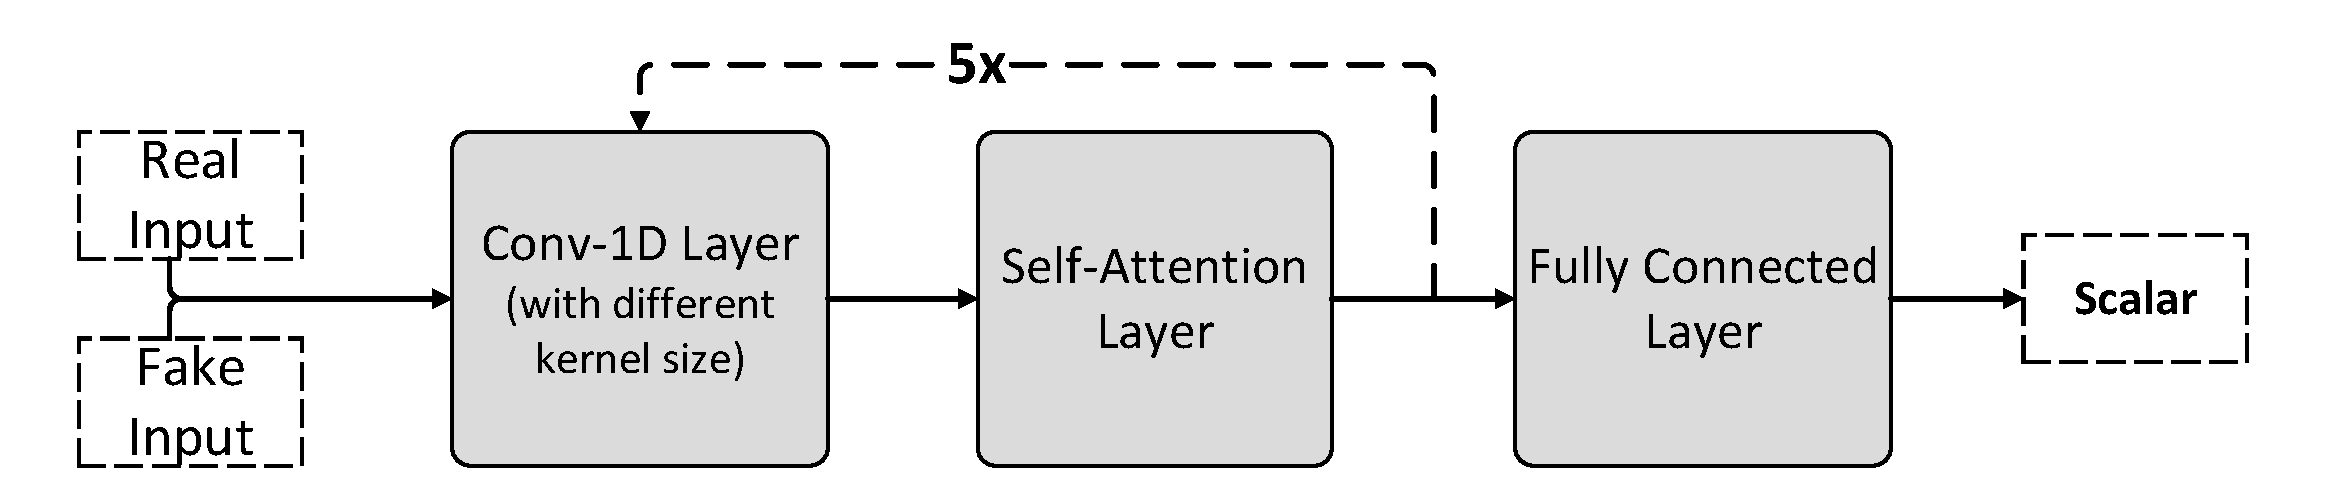
\includegraphics[width=\textwidth]{Figure/FigHexGANFuzzer_Critic.eps}
	\caption{Critic Network}
	\label{FigHexGANFuzzer_Critic}
\end{figure}

It is noted that the first conv-1d layer changes the second dimension of inputs from the probability of word to the feature representation, which is the same as the dimension of NCR. And other conv-1d layers keep the second dimension as $dm$. Every conv-1d layer followed by a self-attention layer but the kernel size of conv-1d is not the same. The kernel size of $i$th conv-1d layer $ks_i = i$ where $i \in \{1,2,3,4,5\}$. 

Protocols have message headers, which specify the content of the message body in the message frame. More simply, the front part of the message frame affects the back part. It is hard to distinguish the boundary of two parts without the knowledge of the protocol grammar. If the model has learned which part is the message header, it can pay more attention to the message header part.
Due to different protocols have different lengths of the message header, the conv-1d layer with different kernel size can capture the information better.

%self-attention layers can capture how flags in the message header affect the part of the message body.
%With the boundary information leaned by conv-1d layers, self-attention layers will pay more attention to the correlation between the content in the message header and body. 

As for the content in the message header, several flags in the message header affect different parts of the content in the message body. Self-attention layers consider the attention weight of every position of the input and is good at learning long-range dependencies. With the boundary information leaned by conv-1d layers, self-attention layers can capture how flags in the message header affect the part of the message body. After repeated self-attention and conv-1d layers five times, the fully connected layer will output a scalar score. The loss of the critic is:
\begin{equation}
L_{c} = \mathop{\mathbb{E}}\limits_{\tilde{x}\sim\mathbb{P}_{g}}\left [ D(\tilde{x}) \right ] 
- \mathop{\mathbb{E}}\limits_{x\sim\mathbb{P}_{r}}\left [ D(x) \right ] 
+ \lambda\mathop{\mathbb{E}}\limits_{\hat{x}\sim\mathbb{P}_{\hat{x}}}\left [ ( \left \| \triangledown_{\hat{x}}D( \hat{x}) \right \|_{2} - 1 )^{2} \right ]
\end{equation}
where $\mathbb{P}_{\tilde{x}}$ defines sampling uniformly along straight lines between pairs of points sampled from the real data distribution $\mathbb{P}_{r}$ and the generator distribution $\mathbb{P}_{g}$. 
In order to satisfy the 1-Lipschitz constraint, the solution of the WGAN-GP model is adopted. 
We use the gradient penalty instead of the weight clipping to enforce the 1-Lipschitz constraint, which leads to a more stable training process.% and the model is easier to train.

\subsubsection{\textbf{Training strategy}}
%Once the model design is completed, we begin to train our model. Under normal circumstances, the training of the GAN is adversarial, which means the generator and discriminator (critic) should be on the same level. If the imbalance is too serious, another one will learn nothing. And this is the reason why the GAN model is difficult to train and the training is unstable.
Due to the properties of the Wasserstein distance, we train the critic better to narrow the Wasserstein distance between fake message frame distribution and real message frame distribution. %, which is the process of improving generator. 
In every epoch, we train generator once and then train the critic $c\_iters$ ($5$ in our model) times. %Adam Optimizer was used both in the generator and the critic. 
In order to judge the convergence of the model, the following equation approximately indicates the value of the Wasserstein distance. If the value of the equation trends to be stable, we consider the model is convergent.
\begin{equation}
W\_distance = 
\mathop{\mathbb{E}}\limits_{x\sim\mathbb{P}_{r}}\left [ D(x) \right ] 
- \mathop{\mathbb{E}}\limits_{\tilde{x}\sim\mathbb{P}_{g}}\left [ D(\tilde{x}) \right ] 
\end{equation}
%Though the model wants to generate the fake message frames that share high similarity to the real message frames, the ulmate goal is to achieve effective fuzzing results and identify as many bugs as possible. In order to obtain the desired results, there should be some differences between the real data and the fake data. So we not only save the final version of the model, which is convergent, but also the intermediate generator model. The model was saved every 10 training epoch deliberately. In such a training strategy, the goal of the high code coverage and deeper testing depth can be achieved.
The model is saved every 10 training epoch deliberately to achieve the goal of the high code coverage and deeper testing depth. Test cases that cause target anomalies will be recollected and put into the training dataset again. Data augmentation and value mutation operation are applied to these data before putting it into the dataset. We assume that retraining the model with these data can improve the capability of the model to discover vulnerabilities.


